    \section{Simulações}

%---------------------------------------------------

\begin{frame}{\textit{Modelo PE}: Processo de simulação}
	
	Dada a seleção do modelo, o seguinte processo é realizado:
	
	\begin{enumerate}
		\item Seleção de constantes e condições iniciais
		\item Método de discretização (RK4)
		\item Plotagem
	\end{enumerate}
\end{frame}


%---------------------------------------------------
\begin{frame}[fragile]
	
	\frametitle{\textit{Modelo PE}: Seleção de constantes}
	    
	\begin{python}
vetor_a = [1, 1, 3]
vetor_b = [
0.5 * (vetor_a[0] - vetor_a[1] - vetor_a[2]),
0.5 * (vetor_a[1] - vetor_a[2] - vetor_a[0]),
0.5 * (vetor_a[2] - vetor_a[0] - vetor_a[1]),
]
c = math.sqrt(3/4)
		
f_inv = 10800
vetor_h = [-1, 0, 0]
vetor_f = [0.1, 0, 0]
g_0 = 8
kappa_0 = 1 / 48
nu_0 = kappa_0
	\end{python}
\end{frame}

%---------------------------------------------------

\begin{frame}{\textit{Método de discretização RK4}: Características gerais}

Um método é de Runge-Kutta explícito de ordem $4$ se, e só se, satisfaz três propriedades:
\begin{enumerate}
    \item Método de passo único explícito;
    \item Apresenta boa estabilidade para equações diferenciais ordinárias (EDOs).
    \item Possui erro global da ordem de $\mathcal{O}(h^4)$, garantindo alta precisão com um custo computacional moderado. 
\end{enumerate}

\end{frame}

%---------------------------------------------------

\begin{frame}{\textit{Método de discretização RK4}: Formulação}

Tomando como referência \cite{roma2023}, podemos expressar o método RK44 da seguinte maneira:
\begin{equation*}
    \Phi(t,y,h) = \frac{1}{6} \left( \kappa_1 + 2\kappa_2 + 2\kappa_3 + \kappa_4 \right) \quad \text{com} \quad
    \begin{cases}
        \kappa_1 = f(t,y) \\
        \kappa_2 = f \left( t + h/2, y + (h/2) \kappa_1 \right) \\
        \kappa_3 = f \left( t + h/2, y + (h/2) \kappa_2 \right) \\
        \kappa_4 = f \left( t + h, y + h\kappa_3 \right)
    \end{cases}
    \end{equation*}
\end{frame}

%---------------------------------------------------
\begin{frame}[fragile]
	
	\frametitle{\textit{Modelo PE}: Condições iniciais - padrão}
	Primeira condição inicial, é a dada por padrão e tem o intuito de reproduzir a figura 1 do artigo.    
	\begin{python}
# Condições iniciais
x0 = [0.1, 0, 0]
y0 = [0.1, 0, 0]
z0 = [0.1, 0, 0]
	\end{python}
\end{frame}

%---------------------------------------------------

\begin{frame}{\textit{Modelo PE}: Resultados condição inicial padrão}
	\begin{figure}
		\centering
		\begin{subfigure}[b]{0.45\textwidth}
			\centering
			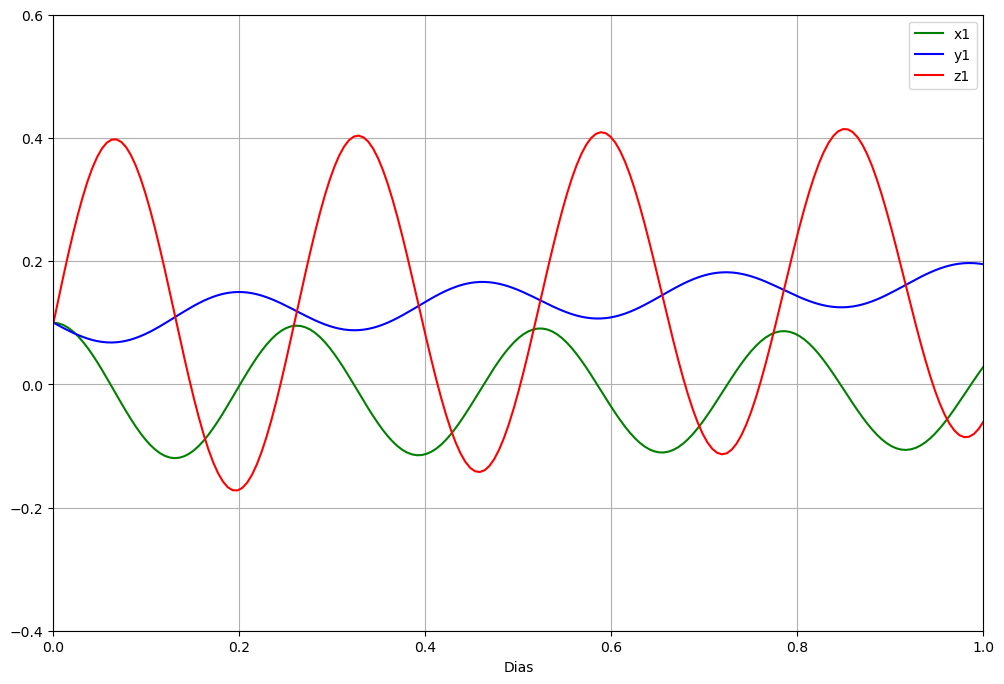
\includegraphics[width=\textwidth]{img/p01d01.png}
			\caption{Condição padrão - 01 dia\\(reprodução)}
			\label{fig:p01d01}
		\end{subfigure}
		\hfill
		\begin{subfigure}[b]{0.45\textwidth}
			\centering
			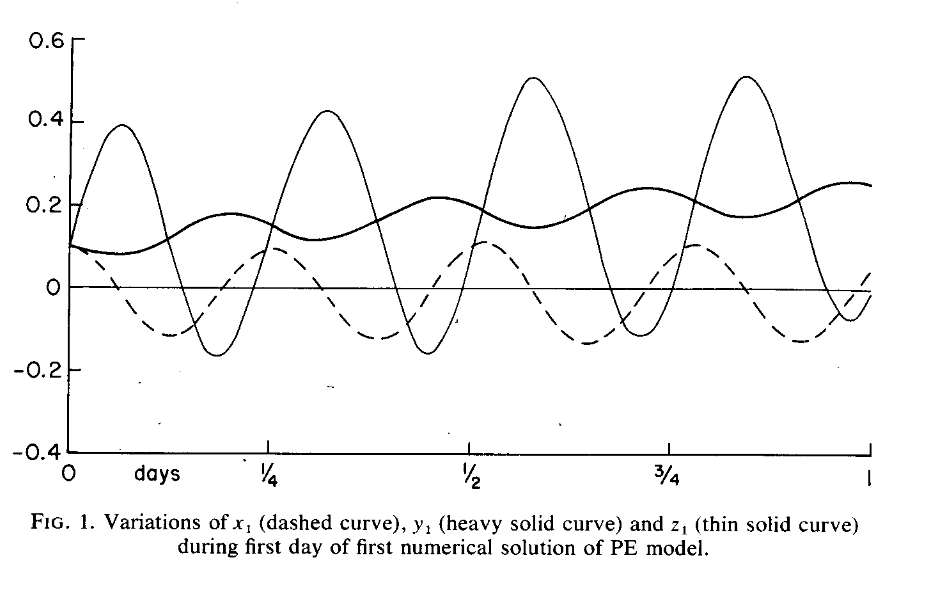
\includegraphics[width=\textwidth]{img/p01d01rel.png}
			\caption{Condição padrão - 01 dia\\(artigo)}
			\label{fig:p01d01rel}
		\end{subfigure}
	\end{figure}
\end{frame}

%---------------------------------------------------

\begin{frame}{\textit{Modelo PE}: Resultados condição inicial padrão}
	\begin{figure}
		\centering
		\begin{subfigure}[b]{0.45\textwidth}
			\centering
			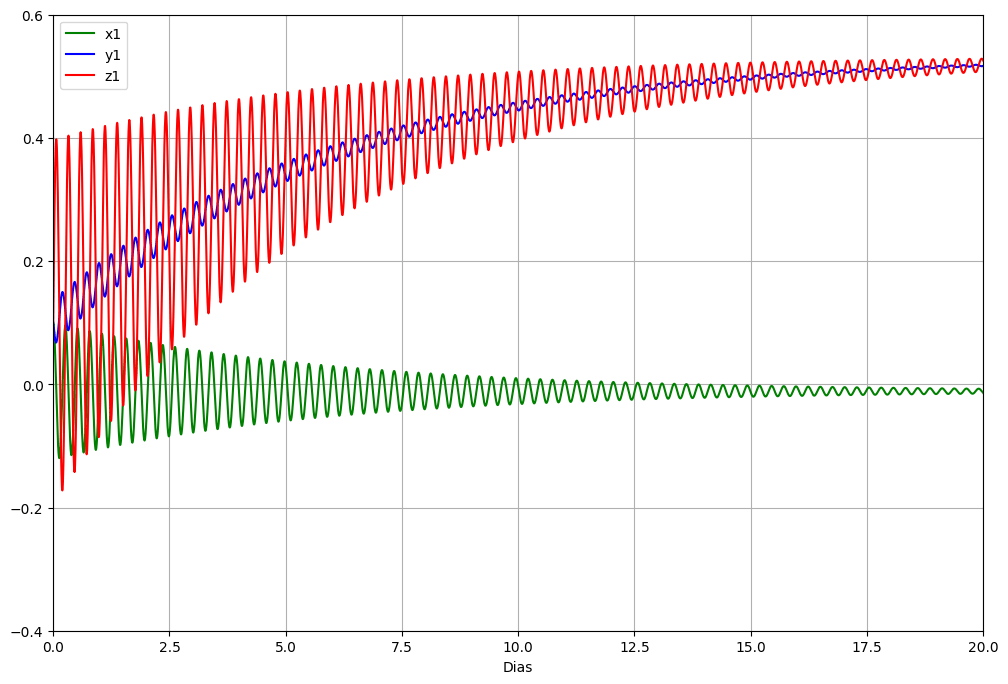
\includegraphics[width=\textwidth]{img/p01d20.png}
			\caption{Condição padrão - 20 dias}
			\label{fig:p01d20}
		\end{subfigure}
		\hfill
		\begin{subfigure}[b]{0.45\textwidth}
			\centering
			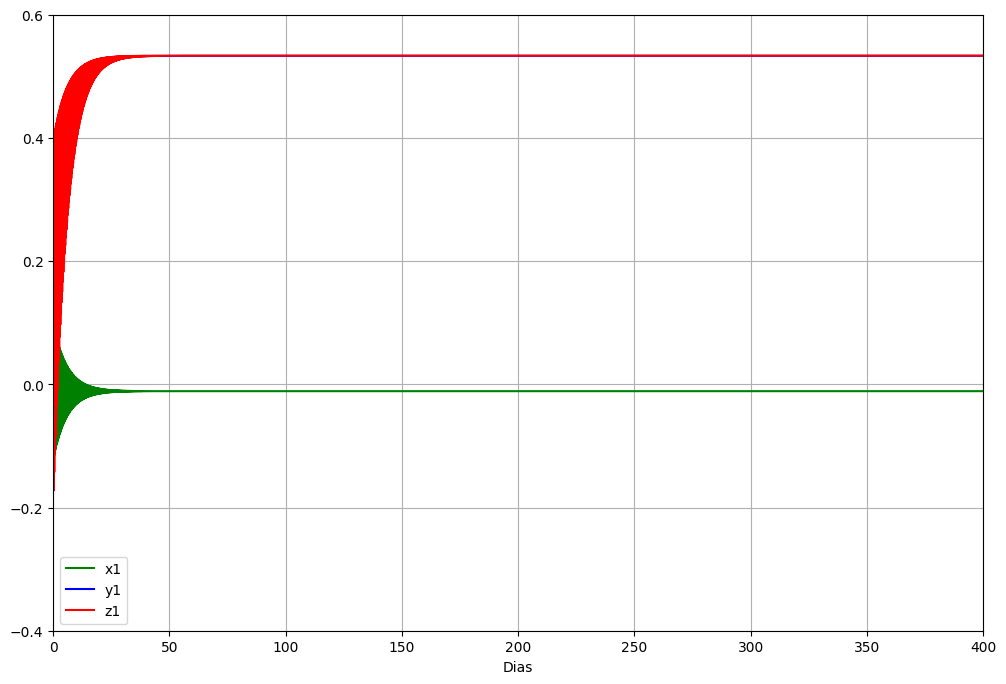
\includegraphics[width=\textwidth]{img/p01d400.png}
			\caption{Condição padrão - 400 dias}
			\label{fig:p01d400}
		\end{subfigure}
	\end{figure}
\end{frame}


%---------------------------------------------------
\begin{frame}{Condições de Hadley}

    A circulação de Hadley é um padrão de circulação atmosférica nos trópicos, onde o ar quente sobe próximo ao equador e desce em latitudes mais altas, formando um ciclo convectivo.
    \begin{itemize}
        \item Em 1735, Hadley incorporou o efeito da rotação da Terra, mostrando que a velocidade do ar varia com a latitude, influenciando a direção predominante dos ventos nos trópicos.
        
        \item Baseia-se na conservação do momento angular, garantindo o equilíbrio do movimento atmosférico e evitando mudanças na rotação da Terra.
        
        \item Responsável pelos ventos predominantes nos trópicos e pela redistribuição de calor na atmosfera, influenciando padrões climáticos globais.
    \end{itemize}
\end{frame}

%---------------------------------------------------

\begin{frame}{\textit{Modelo PE}: Condições iniciais - Hadley 01}
A partir do artigo \cite{gent1982}, temos que os valores dos vetores para as condições de Hadley são definidas como:
	\begin{align*}
        x_1 &= - \nu_0 a_1 y_1, \\
        y_1 &= \frac{F_1}{a_1} v_0 \left( 1 + a_1 g_0 + \nu_0^2 a_1^2 \right), \\
        z_1 &= \left( 1 + \nu_0^2 a_1^2 \right) y_1\\
        x_2 &= y_2 = z_2 = x_3 = y_3 = z_3 = 0
\end{align*}

\end{frame}


%---------------------------------------------------
\begin{frame}[fragile]
	
	\frametitle{\textit{Modelo PE}: Condições iniciais - Hadley 01}
	Adaptando para o código, temos:
	\begin{python}
# Condições iniciais
y1 = (vetor_f[1]
/ vetor_a[1] * nu_0 * (1 + vetor_a[1] * g_0 + nu_0**2 * vetor_a[1] ** 2))
z1 = (1 + nu_0**2 * vetor_a[1] ** 2) * y1
x1 = -nu_0 * vetor_a[1] * y1
		
x_hadley01_inicial = [x1, 0, 0]
y_hadley01_inicial = [y1, -(10 ** (-5)), 0]
z_hadley01_inicial = [z1, 10 ** (-5), 0]
	\end{python}
\end{frame}

%---------------------------------------------------

\begin{frame}{\textit{Modelo PE}: Resultados para condição de Hadley 01}
	\begin{figure}
		\centering
		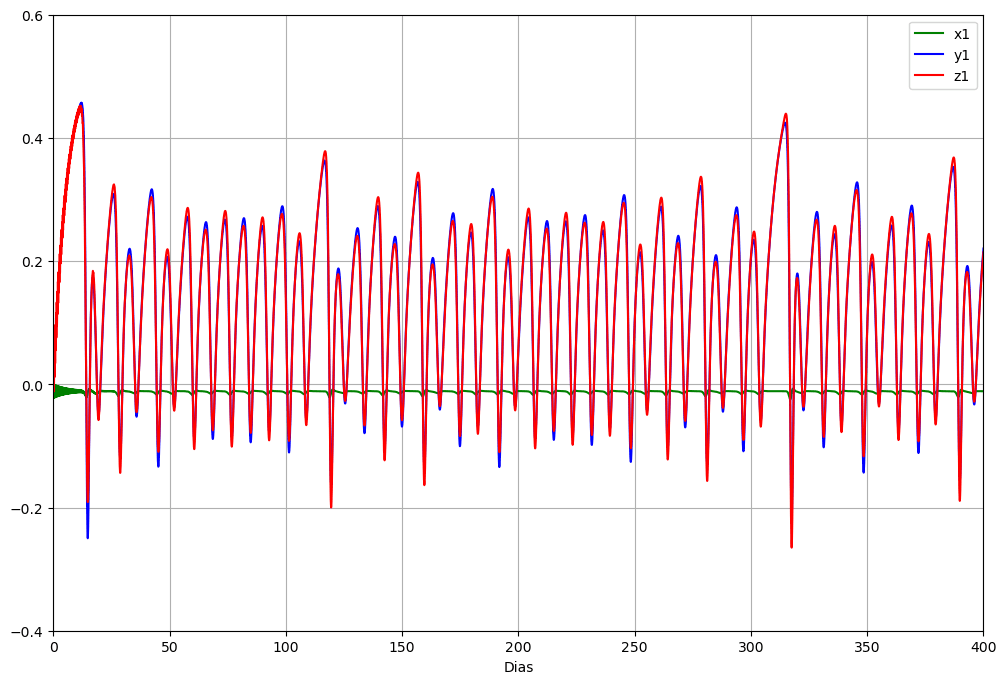
\includegraphics[width=0.5\textwidth]{img/p02d260.png}
		\caption{Hadley 01 - 400 dias}
		\label{fig:p02}
	\end{figure}
\end{frame}

%---------------------------------------------------

\begin{frame}{\textit{Modelo PE}: Resultados para condição de Hadley 01}
	\begin{figure}
		\centering
		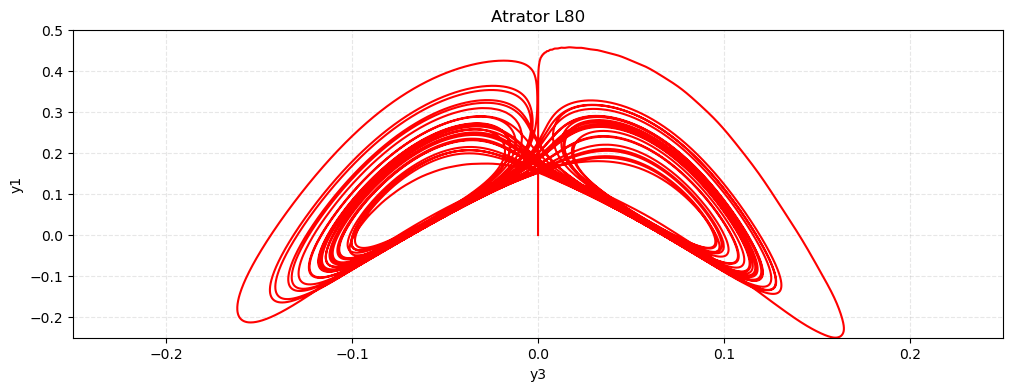
\includegraphics[width=0.7\textwidth]{img/p02y3y1.png}
		\caption{Hadley 01 - Projeção $y_3 \times y_1$}
		\label{fig:p02y3y1}
	\end{figure}
\end{frame}

%---------------------------------------------------

\begin{frame}{\textit{Modelo PE}: Resultados para condição de Hadley 01}
	\begin{figure}
		\centering
		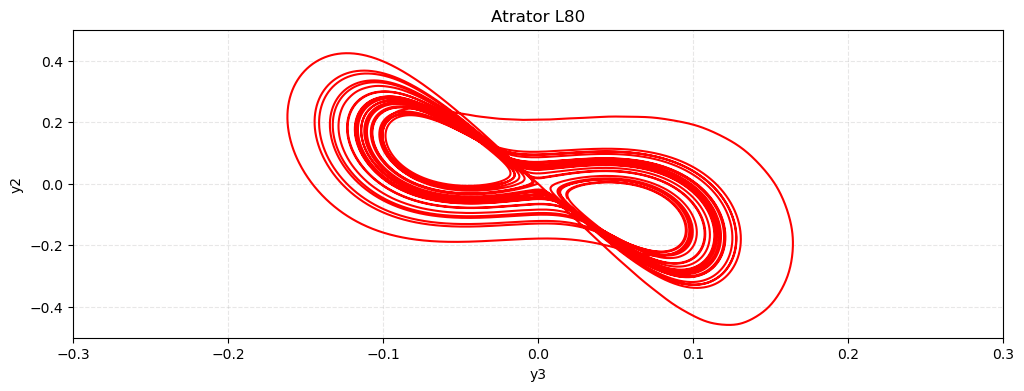
\includegraphics[width=0.7\textwidth]{img/p02y3y2.png}
		\caption{Hadley 01 - Projeção $y_3 \times y_2$}
		\label{fig:p02y3y2}
	\end{figure}
\end{frame}

%---------------------------------------------------

\begin{frame}{\textit{Modelo PE}: Resultados para condição de Hadley 01}
	\begin{figure}
		\centering
		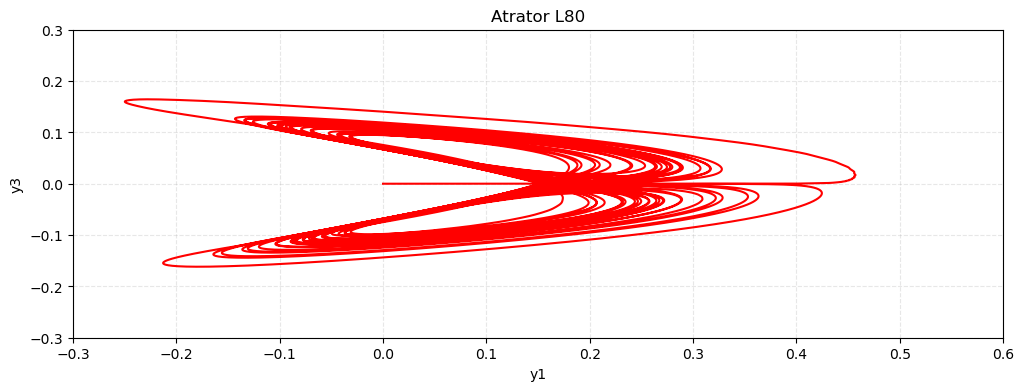
\includegraphics[width=0.7\textwidth]{img/p02y1y3.png}
		\caption{Hadley 01 - Projeção $y_1 \times y_3$}
		\label{fig:p02y1y3}
	\end{figure}
\end{frame}

%---------------------------------------------------

\begin{frame}[fragile]
	
	\frametitle{\textit{PE Model e QG Model}: Condições iniciais - Hadley 02}
	A presente condição reproduz as condições da circulação de Hadley de acordo com \cite{lorenz1980}
	\begin{python}
# Condições iniciais do modelo PE
x_hadley02_inicial = [-0.01111, 0, 0]
y_hadley02_inicial = [0.53331, 0, 0]
z_hardle02_inicial = [0.53354, 0, 0]
	\end{python}
	
	Equivalente a seguinte condição do QG Model:
	\begin{python}
# Condições iniciais do modelo QG
y0 = [0.53333, 0, 0]
	\end{python}
\end{frame}

%---------------------------------------------------

\begin{frame}{\textit{Modelo PE} e \textit{Modelo QG}: Resultados para a condição de Hadley 02}
	\begin{figure}
		\centering
		\begin{subfigure}[b]{0.45\textwidth}
			\centering
			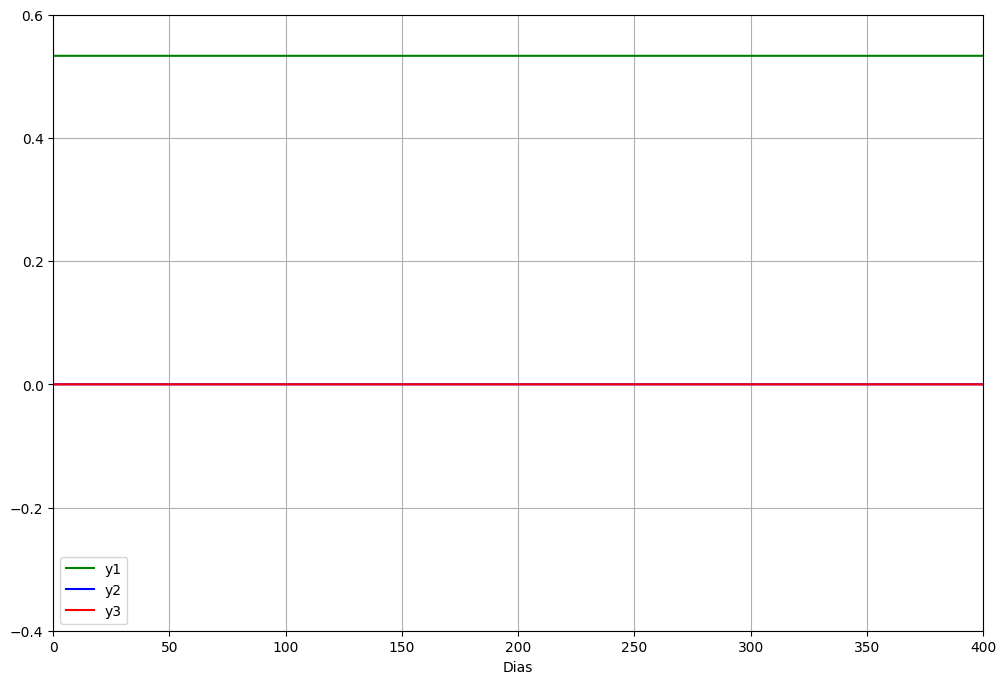
\includegraphics[width=\textwidth]{img/p03d400pe.png}
			\caption{Condição de Hadley 02 - 400 dias\\ (PE Model)}
			\label{fig:p03d400pe}
		\end{subfigure}
		\hfill
		\begin{subfigure}[b]{0.45\textwidth}
			\centering
			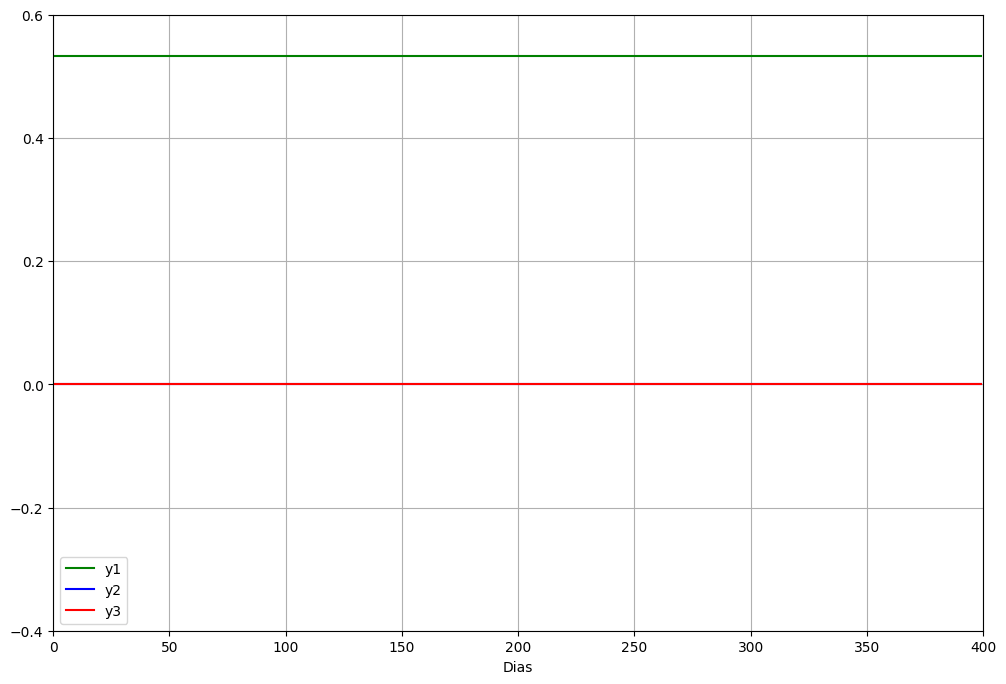
\includegraphics[width=\textwidth]{img/p03d400qg.png}
			\caption{Condição de Hadley 02 - 400 dias\\ (QG Model)}
			\label{fig:p03d400qg}
		\end{subfigure}
	\end{figure}
\end{frame}

%---------------------------------------------------

\begin{frame}{\textit{Algumas dificuldades}: As equações \eqref{eq:equacao-principal-simplificada-1}-\eqref{eq:equacao-principal-simplificada-3}}
	
	\begin{enumerate}
		\item Apesar das equações \eqref{eq:equacao-principal-simplificada-1}-\eqref{eq:equacao-principal-simplificada-3} serem simplificações de \eqref{eq:equacao-principal-1}-\eqref{eq:equacao-principal-3}, nenhuma das referências utilizadas utilizou as equações \eqref{eq:equacao-principal-simplificada-1}-\eqref{eq:equacao-principal-simplificada-3}
		\item Na tentativa de plotagem das \eqref{eq:equacao-principal-simplificada-1}-\eqref{eq:equacao-principal-simplificada-3}, houve diversos problemas, os principais foram: \textit{overflow} e desvio em relação a natureza das equações \eqref{eq:equacao-principal-1}-\eqref{eq:equacao-principal-3}
	\end{enumerate}
\end{frame}

%---------------------------------------------------

\begin{frame}{\textit{Algumas dificuldades}: As equações \eqref{eq:equacao-principal-simplificada-1}-\eqref{eq:equacao-principal-simplificada-3}}
		\begin{figure}
		\centering
		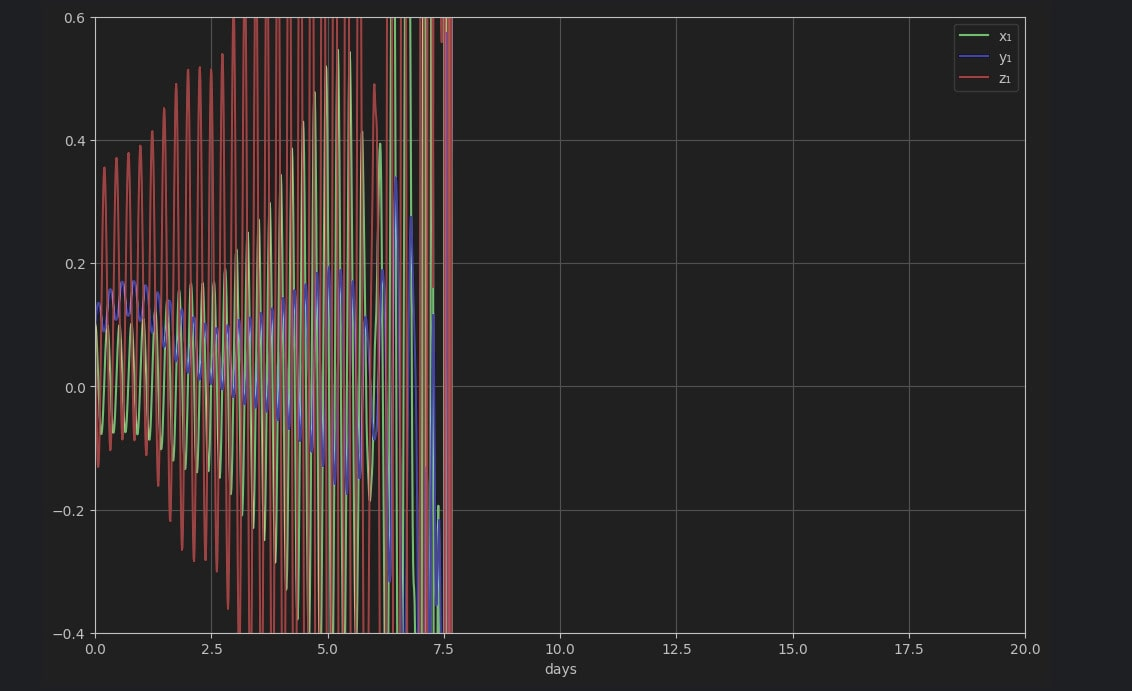
\includegraphics[width=0.5\textwidth]{img/erro_simplificado.jpeg}
		\caption{Tentativa de plotagem equações \eqref{eq:equacao-principal-simplificada-1}-\eqref{eq:equacao-principal-simplificada-3}}
		\label{fig:erro-plotagem-eq-simp}
	\end{figure}
\end{frame}

%---------------------------------------------------

\begin{frame}{\textit{Algumas dificuldades}: equações \eqref{eq:equacao-principal-1}-\eqref{eq:equacao-principal-3}}
	\begin{figure}
		\centering
		\begin{subfigure}[b]{0.45\textwidth}
			\centering
			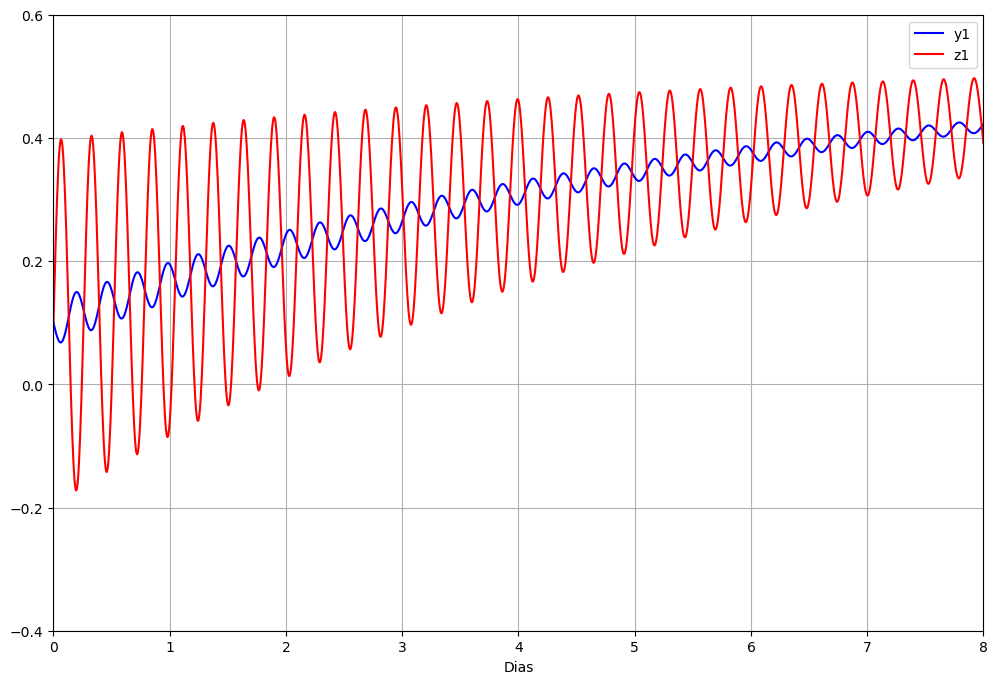
\includegraphics[width=\textwidth]{img/p01d08.png}
			\caption{Condição padrão - 8 dias}
			\label{fig:p01d08}
		\end{subfigure}
		\hfill
		\begin{subfigure}[b]{0.45\textwidth}
			\centering
			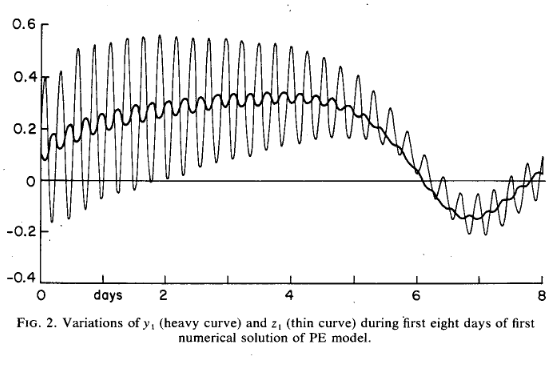
\includegraphics[width=\textwidth]{img/p01d08rel.png}
			\caption{Condição padrão - 8 dias (artigo)}
			\label{fig:p01d08rel}
		\end{subfigure}
	\end{figure}
\end{frame}